\documentclass[preprint,12pt]{elsarticle}

\usepackage{amssymb}
\usepackage{graphics}
\usepackage{float}

\graphicspath{{./Images/}}

\journal{Solar Energy Materials \& Solar Cells}

\begin{document}

\begin{frontmatter}

\title{Life Cycle Analysis of the Adaptive Solar Facade\tnoteref{t1}} 
\tnotetext[t1]{This document is a collaborative effort.} 

\author[ita]{M. Jansen\corref{cor1}}
    \ead{m.jansen@student.ethz.ch}

\author[ita]{P. Jayathissa\corref{cor2}}
    \ead{jayathissa@arch.ethz.ch}

\author[baug]{N. Heeren}
    \ead{heeren@ifu.baug.ethz.ch}

\author[ita]{A. Schlueter}
    \ead{schlueter@arch.ethz.ch}

\author[baug]{S. Hellweg}
	\ead{hellweg@ifu.baug.ethz.ch}

\cortext[cor1]{Corresponding author} 
\cortext[cor2]{Principal corresponding author}

\address[ita]{Architecture and Building Systems, Institute of Technology in Architecture,\\ ETH Zurich, Switzerland} 
\address[baug]{Ecological System Design, Institute of Environmental Engineering,\\ ETH Zurich, Switzerland}

\begin{abstract}
Text text Text textText textText textText textText textText textText textText textText textText textText textText textText textText textText text
\end{abstract}

\begin{keyword}
Adaptive Solar Facade \sep Life Cycle Analysis
\end{keyword}

\end{frontmatter}

\clearpage

\section{Introduction}
\label{introduction}
Through the recent advances in thin film photovoltaic technology 

We are pretty awesome at this

bla bla bla


\section{Life cycle analysis methodology}
\label{method}
% !TEX root = main.tex
The analysis is performed according to ISO14040, ISO14044 and ISO15804

Impact category: GWP

Functional unit: ${\mathrm{m^2}}$ (shading) and ${\mathrm{kWh}}$ (PV)

\begin{equation}
G=\frac{{\mathrm{GWP}}}{{\mathrm{I \cdot \eta  \cdot PR \cdot LT \cdot A}}}
\label{solar}
\end{equation}

Scope and system boundaries: embodied, operational, disposal

\begin{figure}[H]
\begin{center}
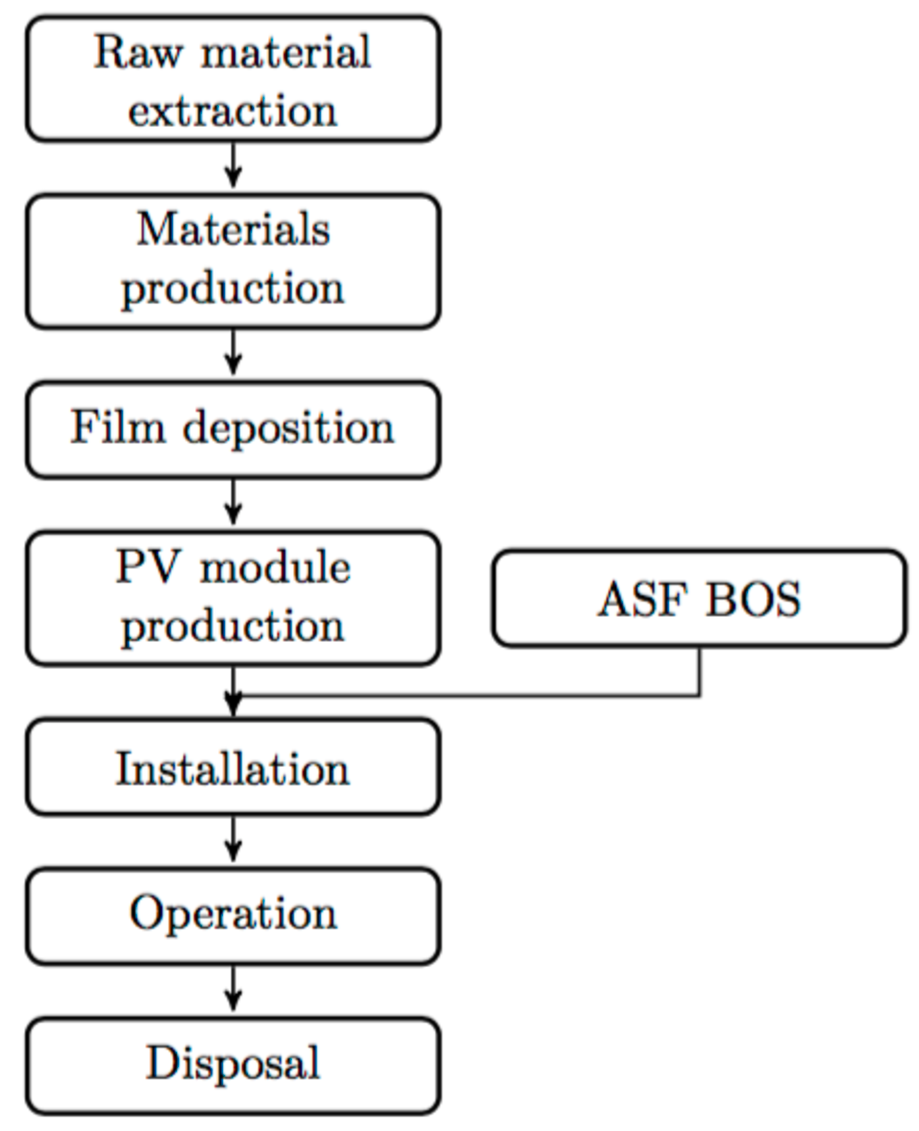
\includegraphics[width=5cm, trim= 0cm 0cm 0cm 0cm,clip]{BOS}
\caption{Thin-film incl. BOS (e.g. supporting structures and systems) analysis}
\label{BOS}
\end{center}
\end{figure}

Cut-off method used

Recipe midpoint H allocation method

\begin{figure}[H]
\begin{center}
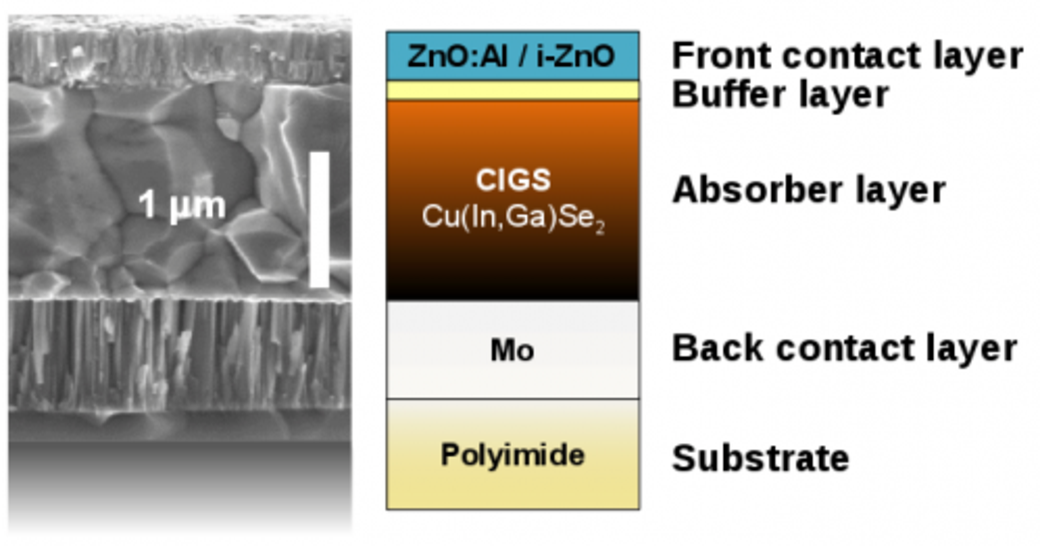
\includegraphics[width=8cm, trim= 0cm 0cm 0cm 0cm,clip]{schema}
\caption{CIGS thin film structure MAKE OWN GRAPH, DO NOT USE THIS ONE FOR FINAL}
\label{schema}
\end{center}
\end{figure}

\begin{enumerate}
\item Solar irradiation Zurich, Switzerland: 1240 ${\mathrm{kWh/m^2/yr}}$
\item Module efficiency CIGS: 11.5\%
\item Performance ratio with optimal algorithm: 0.326\footnote{Based on full facade area of 8.96${\mathrm{m^2}}$; Actual PV film area only comprises of 5.76${\mathrm{m^2}}$}
\item Electricity production: 46.54 ${\mathrm{kWh/m^2}}$; 417 ${\mathrm{kWh}}$
\item Shading office room savings according to Table \ref{simulation} and \ref{netenergy}
\item Lifetime: 15 years
\item Maintenance every 5 years: 69.9 ${\mathrm{kg_{CO_2eq}}}$\footnote{Includes: baking and vacuuming actuator, actuator silicone, actuator mold and idling hoist for 8 hours}
\item Disposal processes according to Appendix \ref{}
\item Database source: Ecoinvent 3.1
\end{enumerate}

\section{Adaptive solar facade environmental profile}
\label{profile}
% !TEX root = main.tex

- The results of the analysis can be summarized in Figure \ref{fig:waterfall}...

\begin{figure}[H]
\begin{center}
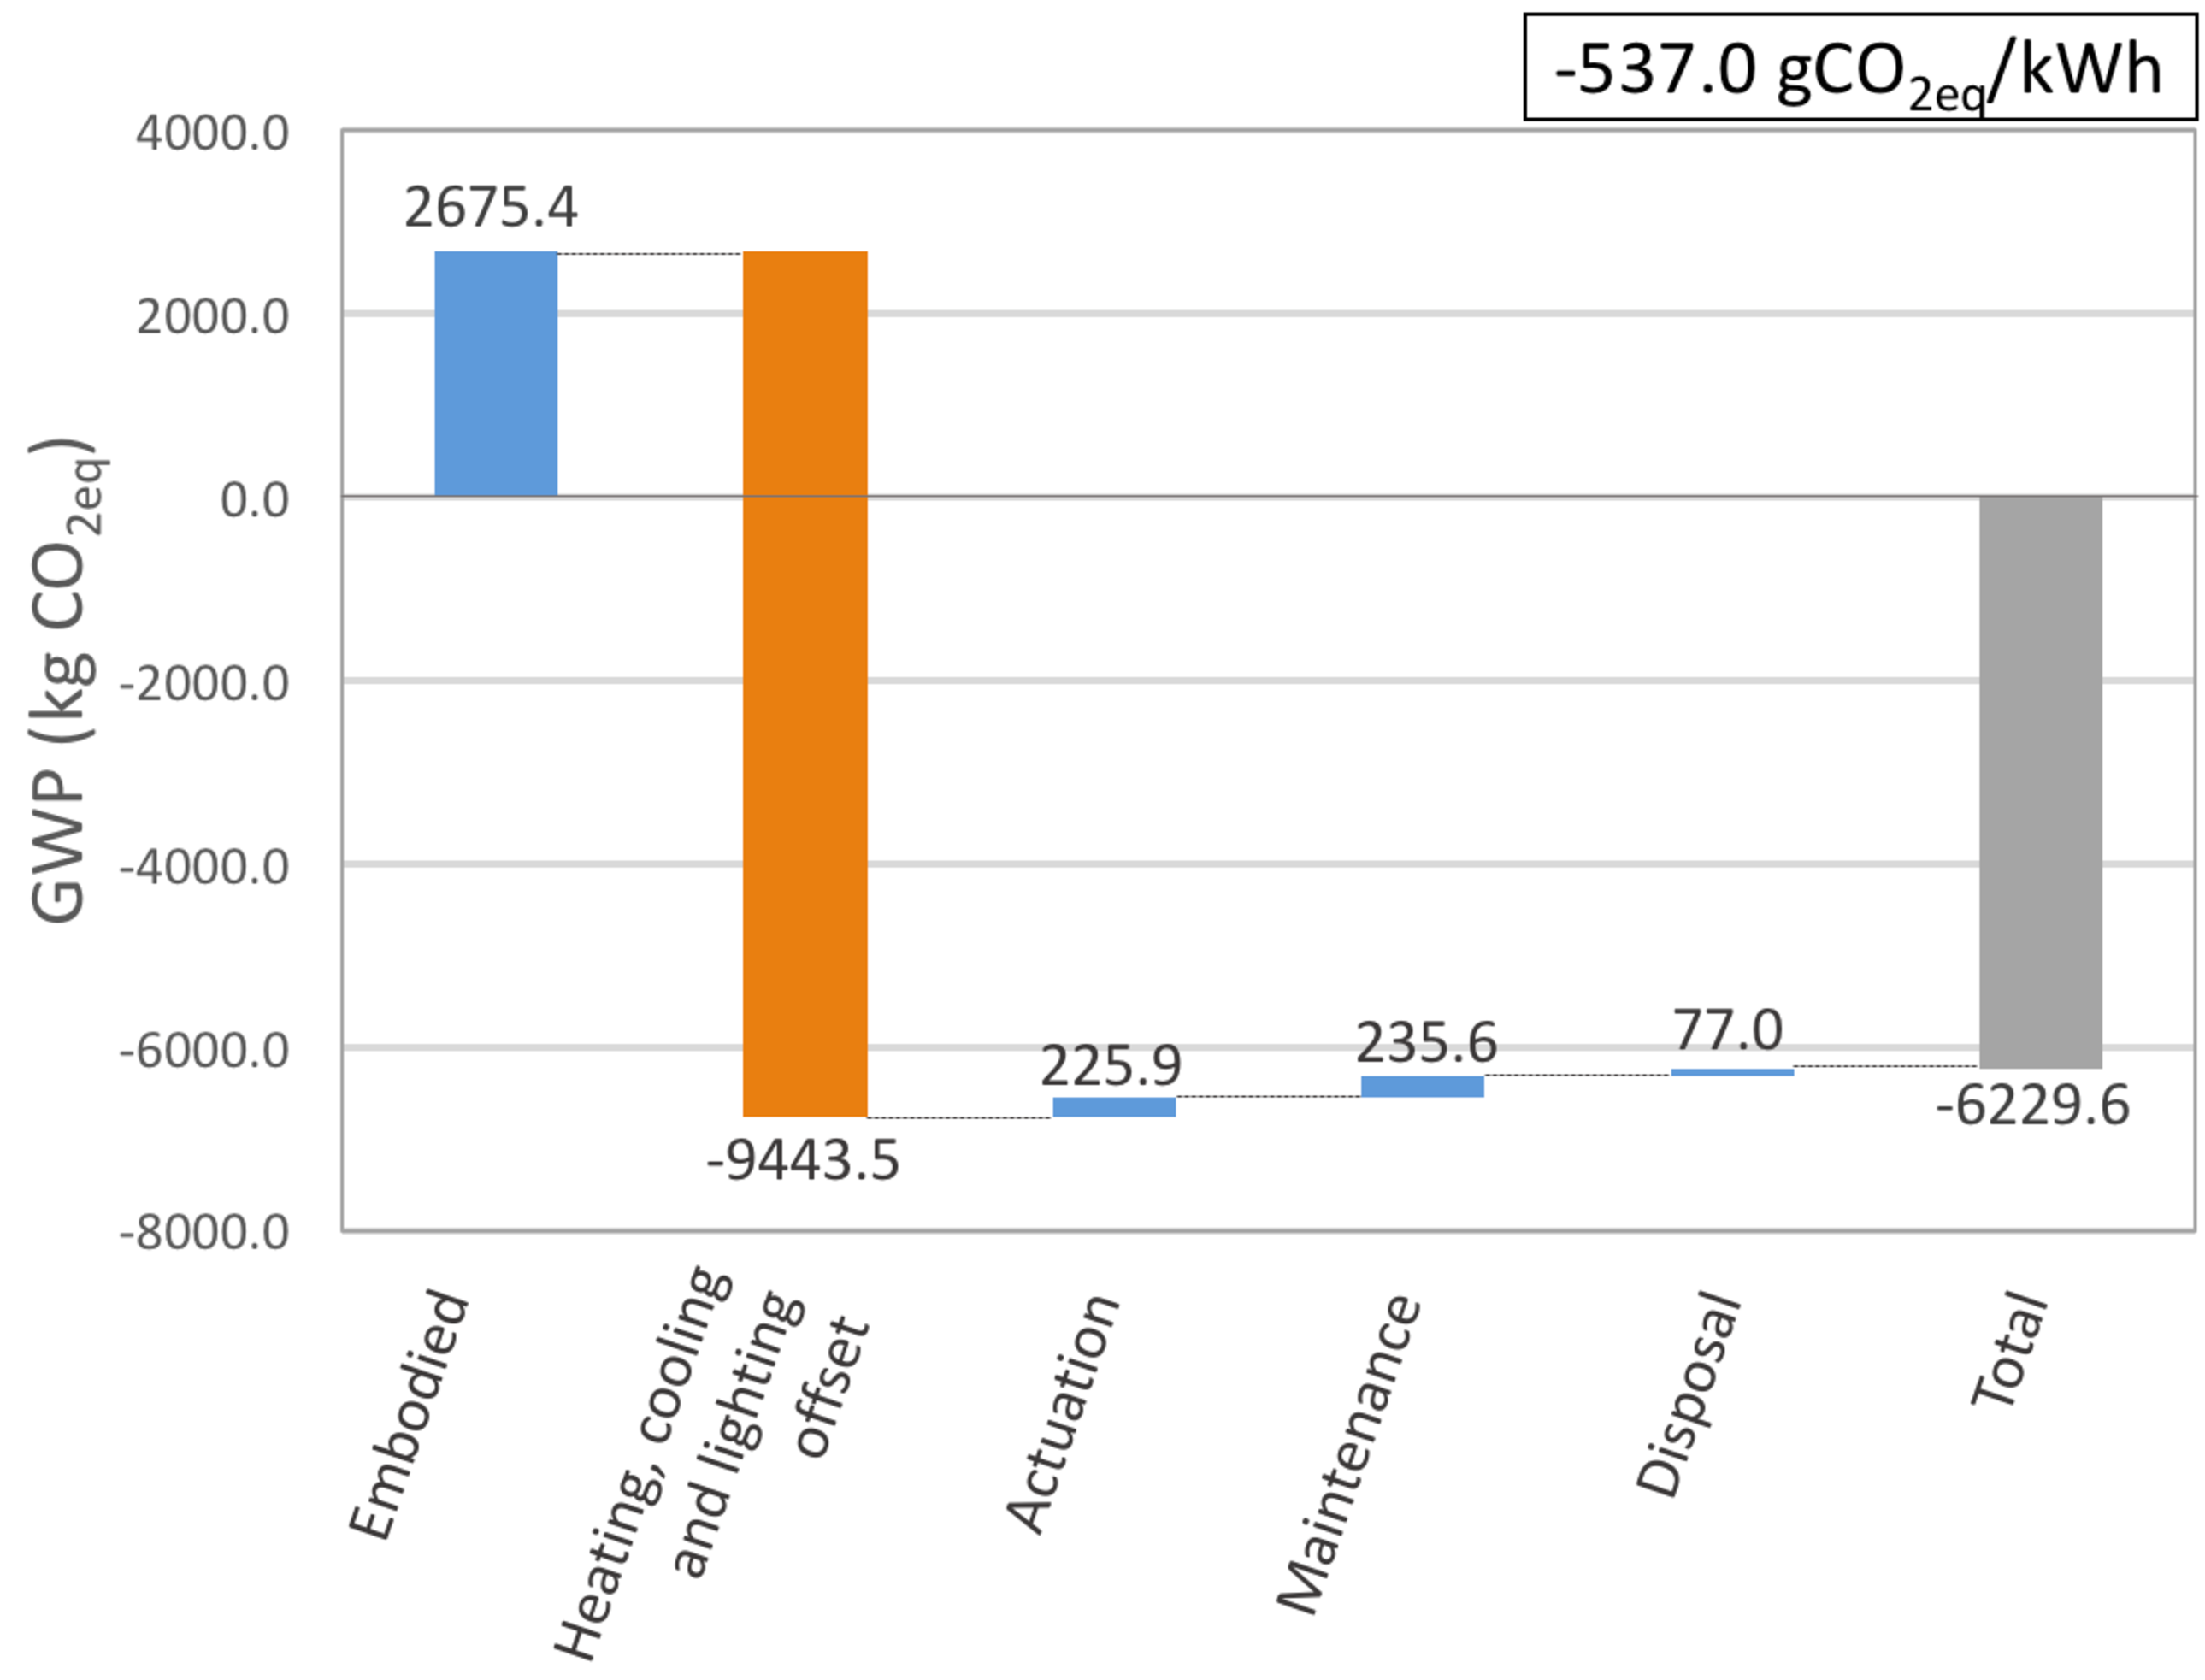
\includegraphics[width=10cm, trim= 0cm 0cm 0cm 0cm,clip]{waterfall}
\caption{Breakdown of GWP of the ASF into embodied, operational and disposal emissions}
\label{fig:waterfall}
\end{center}
\end{figure}

- A breakdown of the embodied carbon emissions can be found in Figure  \ref{fig:embodied}... (brief discussion and design consideration)...

\begin{figure}[H]
\begin{center}

\includegraphics[width=10cm, trim= 0cm 0cm 0cm 0cm,clip]{embodied}
\caption{Breakdown of the embodied carbon emissions, it can be seen that xxxx has the greatest GWP contribution}
\label{fig:embodied}
\end{center}
\end{figure}



- As input parameters of production processes are stochastic, a Monte Carlo simulation is used to include this stochastic behavior in the results, as shown in Figure \ref{fig:monte}...

\begin{figure}[H]
\begin{center}

\includegraphics[width=10cm, trim= 0cm 0cm 0cm 0cm,clip]{monte}
\caption{Monte carlo simulation based on input uncertainties}
\label{fig:monte}
\end{center}
\end{figure}

- Sourcing location greatly influences the embodied GWP. For photovoltaic panels, the majority of embodied emissions result from the use of electricity during production. The GWP per kwh of the Chinese electricity mix is 1145.8 ${\mathrm{gCO_2eq/kWh}}$, while in Switzerland this is only 119.6 ${\mathrm{gCO_2eq/kWh}}$.

\begin{figure}[H]
\begin{center}

\includegraphics[width=10cm, trim= 0cm 0cm 0cm 0cm,clip]{sensitivity}
\caption{Sensitivity analysis based on sourcing location}
\label{fig:sensitivity}
\end{center}
\end{figure}


\section{Comparison to other technologies}
\label{comparison}
% !TEX root = main.tex

- The adaptive solar facade was compared with standard facade shading systems and other static BIPV solutions...

\begin{figure}[H]
\begin{center}
\includegraphics[width=10cm, trim= 0cm 0cm 0cm 0cm,clip]{louvres}
\caption{Shading system comparison}
\label{fig:louvres}
\end{center}
\end{figure}

\begin{figure}[H]
\begin{center}
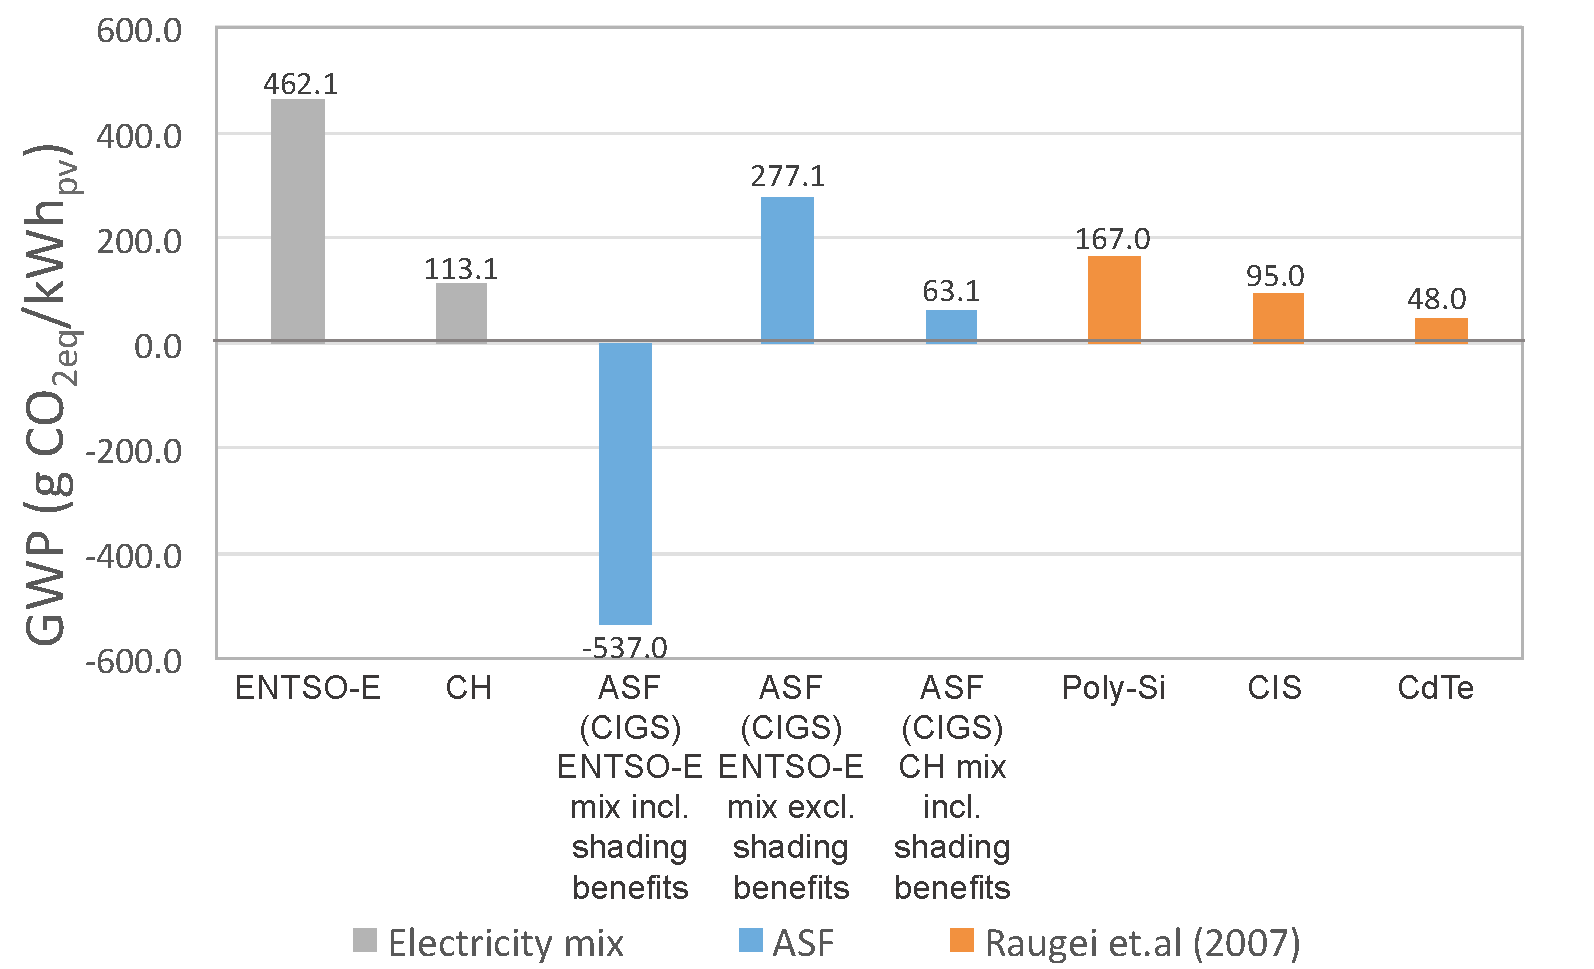
\includegraphics[width=10cm, trim= 0cm 0cm 0cm 0cm,clip]{compPV}
\caption{BIPV comparison of thin-film and BOS}
\label{fig:compPV}
\end{center}
\end{figure}

\section{Conclusion}
\label{conclusion}
% !TEX root = main.tex

- xxx\% of Embodied emissions of the photovoltaic BOS can be offset through smart shading
- This multi functionality brings about new advantages/disadvantages for solar as it has a reduced/increased BOS emissions rate
- Higher embodied CO2 compared to a classic photovltaic retrofit. However reduction can be made through x y and z
- Results are highly sensitive to x y and z


\section{Acknowledgments}
\label{acknowledgments}
...

%% appendix sections are then done as normal sections
%% \appendix
%% \section{}
%% \label{}

%% bibitems, please use
%%  \bibliographystyle{elsarticle-num} 
%%  \bibliography{<your bibdatabase>}

\end{document}
\endinput